
\section{بیان مسئله }\label{sec1}


اندازه‌گیری دقیق ضربان قلب یکی از مهم‌ترین مسائل در علم پزشکی است که برای نظارت بر سلامت افراد، به ویژه در محیط‌های بیمارستانی و کلینیکی، کاربرد گسترده‌ای دارد. روش‌های سنتی اندازه‌گیری ضربان قلب نظیر الکتروکاردیوگرام (\lr{ECG}) و پالس اکسیمتر به طور معمول به تماس فیزیکی با بدن نیاز دارند، که ممکن است باعث محدودیت‌هایی برای بیمار شود و همچنین نیاز به تجهیزات جانبی داشته باشد. علاوه بر این، این روش‌ها در محیط‌هایی که بیمار در حال حرکت است یا در شرایط دشوار نظیر محیط‌های بیمارستانی شلوغ، دقت کمتری دارند.
در این راستا، استفاده از تکنولوژی‌های جدیدی مانند رادارهای \lr{FMCW (Frequency Modulated Continuous Wave)} به عنوان یک راهکار جایگزین مطرح می‌شود. این رادارها با بهره‌گیری از امواج رادیویی می‌توانند حرکت‌های بدن انسان را شبیه‌سازی کرده و حتی تغییرات کوچک در موقعیت بدن مانند ضربان قلب را شبیه‌سازی و اندازه‌گیری کنند. استفاده از رادارهای \lr{FMCW} در اندازه‌گیری ضربان قلب این مزیت را دارد که به هیچ‌گونه تماس فیزیکی نیاز ندارد و قادر است در محیط‌هایی که حرکت یا موانع فیزیکی وجود دارد، با دقت بالا ضربان قلب را اندازه‌گیری کند.
این تحقیق بر استفاده از رادارهای \lr{FMCW} برای اندازه‌گیری ضربان قلب تمرکز دارد و هدف آن ارزیابی کارایی این تکنولوژی در شرایط مختلف است. با توجه به مزایای رادارهای \lr{FMCW}، از جمله حساسیت بالا به حرکت‌های کوچک و قابلیت عملکرد در شرایط غیرتماسی، این تحقیق می‌تواند به‌عنوان یک راهکار در زمینه پایش سلامت انسان در محیط‌های مختلف، به ویژه در مراقبت‌های پزشکی از راه دور و پزشکی دیجیتال، معرفی گردد.

\vspace{2cm}
\begin{center}
\begin{figure}[!h]
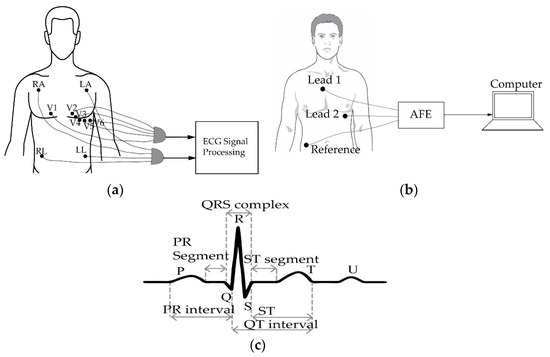
\includegraphics[height=7cm,width=12cm]{Images/chapter1/1-1.jpg}
\caption{(الف) سیستم الکتروکاردیوگرام بالینی؛ (ب) سیستم الکتروکاردیوگرام قابل حمل؛ (ج) نمایش سیگنال \lr{ECG}.\cite{kebe2020human}
}
\end{figure}
\end{center}
\vspace{2cm}

